
\def\1{\y1}
\def\2{\y2}
\def\3{\y3}
\def\4{\y4}
\def\5{\y5}
\def\6{\y6}
\def\7{\y7}
\def\8{\y8}
\def\9{\y9}
\def\0{\y0}
\def\-{\y-}
\aaa{Real Quadratic Form and symmetric matrices}

Suppose you are working with polynomials $\{a+bx : a,b ∈ ℝ \}$, and you see a note on the table claiming that they have defined an inner product to this space by
$$
‹1,1› = 2; ␣ 
‹1,x› = 3; ␣ 
‹x,x› = 5
$$

You wonder how this inner product being defined?
\a\aa
Your frinend tells you that their method is let
$$
f(x) ↦  \m {f(1)},{f(2)}.
$$
so that they define $‹f,g›=f(1)g(1)+f(2)g(2)$.
\vfill
Why not $f(1)g(1)+f(3)g(3)$??? Why not $f(7)g(7)+f(2)g(2)$???
\a\aa

In ℝ^n, We have inner product defined by

$$
‹\vec v,\vec w› = \vec v^T\vec w
$$
Explicitly,
$$
‹\m{x_1},{x_2},\vdots,{x_n}.,
\m{y_1},{y_2},\vdots,{y_n}.›
=x_1y_1+x_2y_2+\cdots+x_ny_n.
$$

Is this the only possible inner product?

\a{Try to classify inner product}
Inner product satisfies 
$$ ‹λ\vec v+μ\vec u,\vec w›  = λ‹\vec v,\vec w›+μ‹\vec u,\vec w›.  $$
$$‹\vec v,\vec u› = ‹\vec u,\vec v›$$
\[defi]{ Call a function $‹-,-›:ℝ^n × ℝ^n ⟶  ℝ $ a \x{bilinear symmetric form} if it is 
\[enumerate]{
\item symmetry: $‹\vec v,\vec w› = ‹\vec w,\vec v›$;
\item bilinear:\[itemize]{\item $ ‹λ\vec v+μ\vec u,\vec w›  = λ‹\vec v,\vec w›+μ‹\vec u,\vec w›$ \item and $    ‹\vec v,λ\vec w+μ\vec u›=λ‹\vec v,\vec u›+μ‹\vec v,\vec w›$}
}
}


\a\aa
Furthermore, as an inner product, we must have $‹v,v› > 0$ for any $v≠0$;
\[defi]{ Call a function $‹-,-›:ℝ^n × ℝ^n ⟶  ℝ $ an \x{inner product} if it is 
\[enumerate]{
\item symmetry: $‹\vec v,\vec w› = ‹\vec w,\vec v›$;
\item bilinear:\[itemize]{\item $ ‹λ\vec v+μ\vec u,\vec w›  = λ‹\vec v,\vec w›+μ‹\vec u,\vec w›$ \item and $    ‹\vec v,λ\vec w+μ\vec u›=λ‹\vec v,\vec u›+μ‹\vec v,\vec w›$}
\item \x{positive definite}: For any non-zero vector $\vec v$, we have $‹\vec v,\vec v› >0$.
}
}
In other words, an inner product is a \x{positive deifnite} bilinear symmetric form.

\a{Classification of bilinear form}
We have a way to construct bilinear form:
$$
‹\vec v,\vec w›_A := \vec v^TA\vec w
$$

Our inner product is a special case when $A = I_n$.

Note that $‹e_i,e_j›_A=e_i^TAe_j$ is the entry of $A$ at i'th row and j'th column, we may view $A$ as the matrix
$$
A = \m
{‹e_1,e_1›_A}
{‹e_1,e_2›_A}
\cdots
{‹e_1,e_n›_A},
{‹e_2,e_1›_A}
{‹e_2,e_2›_A}
\cdots
{‹e_2,e_n›_A},
\vdots
\vdots
\ddots
\vdots,
{‹e_n,e_1›_A}
{‹e_n,e_2›_A}
\cdots
{‹e_n,e_n›_A}.
$$
The matrix $A$ is the value table of inner products for vectors in natural basis. \x{Every bilinear form can be written as} $
‹\vec v,\vec w›_A := \vec v^TA\vec w
$



\a\aa

We have natural way of constructing positive definite bilinear form 
$$
‹\vec v,\vec w›_{M^TM} = ‹ Mv, Mw ›
$$

If $M$ is \li, then $v≠0 ⟺  Mv≠0$. Therefore, for any $v≠0$, we have
$$
‹Mv,Mv› > 0 
$$

If $M$ is a general matrix with columns might not linearly independent, we have
$$
‹Mv,Mv›≥0.
$$
\a\aa
\[defi]{A bilinear form $‹-,-›: ℝ^n × ℝ^n ⟶   ℝ $ is called \x{positive semi-definite} if
$$
‹v,v›≥0 “ for all “v ∈ ℝ^n
$$
furthremore it is called \x{positive definite} if
$$
‹v,v›>0 “ for all “0≠v ∈ ℝ^n
$$
}
\[prop]{
The form $‹-,-›_{M^TM}$ defined by $‹\vec v,\vec w›_{M^TM} := ‹ Mv, Mw › = v^TM^TMw$ is always \x{positive semi-definite}, and
$$
‹-,-›_{M^TM} “ positive definite “ ⟺   “columns of M linearly independent“
$$
}
\a\aa
\[defi]{We call a symmetric matrix $A$ positive semi-definite (resp. definite) if its bilinear form $‹-,-›_A$ is semi-definite (resp. definite). In other words
$$ A “ positive semi-definite “ ⟺  v^TAv ≥0 “ for all “v $$
$$ A “ positive definite “ ⟺  v^TAv >0 “ for all “v≠0 $$
}




\aaa
\aaa{Unit ball of bilinear form}
Call the set
$$
\{v ∈ ℝ^n:‹v,v›=1\}
$$
the unit ball of the bilinear form $‹-,-›$.

\a\aa
Let's visualise unit balls in ℝ^2.

Unit ball of positive definite form $\m{\frac14}0,01.$defines an eclipse. 



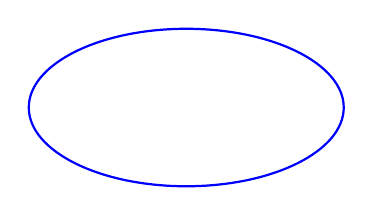
\begin{tikzpicture}
    \draw[thick,blue] (0,0) ellipse (2cm and 1cm);
\end{tikzpicture}


Unit ball of semi-positive definite form $\m00,01.$

\begin{tikzpicture}
    \draw[thick,blue] (-4,1)--(4,1);
    \draw[thick,blue] (-4,-1)--(4,-1);
\end{tikzpicture}
\a\aa
Unit ball of indefinite form $\m{-1}0,01.$. Vectors on the asymptotes have length $0$.


\begin{tikzpicture}
    \draw[blue,thick,scale=1, domain=-1.5:1.5, smooth, variable=\t]
        plot ({sinh(\t)}, {cosh(\t)}) 
        plot ({sinh(\t)}, {-cosh(\t)}); % The other half of the hyperbola
     \draw[thick,dotted] (-3,-3)--(3,3);
     \draw[thick,dotted] (3,-3)--(-3,3);
%    \draw[->] (-3,0) -- (3,0) node[right] {$x$}; % x-axis
%    \draw[->] (0,-3) -- (0,3) node[above] {$y$}; % y-axis
\end{tikzpicture}

\a\aa

\[rem]{In general references, whenever they say \x{positive definite}, \x{positive semidefinite}, or \x{indefinite}, we automatically refers to symmetric matrices. }

\aaa
\aaa{Properties of Positive Semi-definite matrices}
\[prop]{
The \x{sum} of two symmetric \x{positive semidefinite} matrix is again \x{symmetric positive semi definite}, if one of them is \x{definite}, then the \x{sum is definite} as well.
}

\textbf{Proof}:Let $A$ and $B$ be semi-definite. For any $v$, 
$$ v^T(A+B)v = v^TAv+v^TBv ≥ 0+0=0.$$
  If one of them is definite, then $$v^T(A+B)v = v^TAv+v^TBv > 0+0=0.$$

\a\aa

Last lecture,  every symmetric matrix $A$ can be written as
$$
A = Ω^HΛΩ.
$$
with $Ω^HΩ=I_n$. We have
$$
A = A^T ⟹   Λ = Λ^H ⟹   Λ = ¯Λ ⟹   A “ has real eigenvalues“.
$$

\a\aa
\[lem]{A diagonal matrix is \x{positive definite} if and only if all diagonal entries is \x{positive}, and \x{semi-definite} if and only if all diagonal entries is \x{non-negative}.
}
Suppose
$$
Λ=\m
{λ_1}{}{}{},
{}{λ_2}{}{},
{}{}\ddots{},
{}{}{}{λ_n}.
$$
Let $e_i$ be the $i$'th column of identity matrix, then
$$
e_i^TΛe_i = λ_i
$$
So $Λ$ positive semi-definite ⟹   λ_i≥0. $Λ$ positive definite ⟹   $λ_i>0$
\a\aa
On the contary, if $λ_i≥0$ for all $i$, then for any non-zero vector $\vec v=\m{x_1}\cdots{x_n}.^T$, 
$$
\vec v^TΛ\vec v = λ_1x_1^2+λ_2x_2^2+…+λ_nx_n^2 ≥0
$$
Furthermore, if $λ_i>0$, then we have  
$$λ_1x_1^2+λ_2x_2^2+…+λ_nx_n^2 >0.$$
\a\aa
\[lem]{Suppose $Ω$ is an invertible matrix and $A= Ω^TΛΩ$, then $A$ is positive semi-definite or definite if and only if $Λ$ is.}
$$
v^TAv =v^TΩ^TΛΩv = (Ωv)^TΛ(Ωv).  ␣  
$$
$$ Λ“ positive semi-definite “ ⟹   A“ positive semi-definite “ $$
Because $v≠0 ⟹  Ωv≠0$, then 
$$ Λ“ positive definite “ ⟹   A“ positive definite “ $$
$$
v^TΛv =v^T(Ω^{-1T}ΛΩ^{-1})v = (Ω^{-1}v)^TA(Ω^{-1}v).  ␣
$$
$$
A“ positive semi-definite “ ⟹   Λ“ positive semi-definite “
$$
similarly, because $v≠0 ⟹  Ω^{-1}v≠0$, then
$$ A“ positive definite “ ⟹   Λ“ positive definite “ $$
\a\aa

\[thm]{A symmetric matrix $A$ is positive semi-definite if and only if all its eigenvalue are non-nogative, it is positive definite if and only if all its eigenvalue are positive.
}


\[thm]{
A semi-positive definite matrix $A$ is positive definite if and only if and only if it is \x{invertible}.
}

\aaa
\aaa{Positive semi-definite form and Cauchy Inequality}
Let $A$ be a semi-positive definite symmetric matrix, it defines an inner product
$$
‹x,y› = x^TAy.
$$

\[thm]{For any semi-positive definite symmetric matrix $A$, we have Cauchy Inequality
$$
‹x,y›_A^2 ≤ ‹x,x›_A‹y,y›_A
$$}
\a\aa
The geometric intuition of Cauchy inequality can be viewed as follows. Let us consider the case where $A=I$. Take square root, the Cauchy inequality can be written as $‹x,y› ≤ \sqrt{‹x,x›}\sqrt{‹y,y›}$ Then this inequality can be written as
$$
‹\frac x{\sqrt{‹x,x›}},\frac y{\sqrt{‹y,y›}} › ≤1.
$$
In orther words, it means the dot product of two unit vector must be less than $1$.

Geometrically, the dot product of a vector with another unit vector is the length of projection

\[z]{
\draw[thick,blue,->] (0,0) -- (0.7,0.7);
\draw[thick,blue,->] (0,0) -- (1,0);
\draw[thick,blue] (0,0) circle[radius=1];
\draw[thick,red] (0,0.02) -- (0.7,0.02);
\draw[thick,red,dotted] (0.7,0.7) -- (0.7,0);
}
\a\aa
\textbf{Proof of Cauchy inequality}
If ‹x,x›_A≠0, then $‹x,x›_A>0$ consider the vector defined by
$$
w=‹x,x›_Ay - ‹x,y›_Ax
$$
We have
$$
‹w,w›_A = ‹‹x,x›_Ay, ‹x,x›_Ay› - ‹‹x,x›_Ay, ‹x,y›_Ax› 
$$
$$- ‹ ‹x,y›_Ax ,‹x,x›_Ay ›  +‹ ‹x,y›_Ax, ‹x,y›_Ax›
$$
Simplify this expression we have
$$
0≤‹w,w›_A =‹x,x›_A^2‹y,y›_A -  ‹x,y›_A^2‹x,x›_A
$$
Divide both sides by $‹x,x›_A$, we have
$$
0≤ ‹x,x›_A‹y,y›_A -  ‹x,y›_A^2
$$
\a\aa
The Cauchy inequality also holds for ‹y,y›_A≠0 by symmetry.
We have left over a case if $‹x,x›_A=‹y,y›_A=0$. In this case,
$$
0≤ ‹x+ay,x+ay› = 2a‹x,y›
$$
for all $a$, therefore, we must have $‹x,y›=0$, the inequality holds.
\aaa
\aaa{Cauchy Inequality and Cross Filling}
Now we study methods of verifying positive semi-deinity. 

\a\aa
\[prop]{If $A$ is a symmetric positive semi-definite matrix, then all its diagonal entries must be non-negative.}
This is because that the diagonal entry is given by $e_i^TAe_i$.
\a\aa


\[prop]{If $A$ is a positive semi-definite matrix and there is a number $0$ on diagonal of $A$, then the entire row and column containing that diagonal 0 will be 0.}

$$
\m *****,*****,**0**,*****,*****. ⟹   \m
**0**,
**0**,
00000,
**0**,
**0**.
$$
This is to prove $‹e_i,e_i›_A=0$ ⟹   $‹e_i,e_j›_A=0$, this follows from Cauchy's inequality for semi-definite matrix.
\a\aa
Explain why the following symmetric matrix is NOT positive semi-definite?
$$
\m 12{-3},202,{-3}25.
␣ 
\m 12{-3},222,{-3}2{-1}.
$$
\a\aa
\[cor]{Let $A$ be a symmetric matrix with all diagonal entries equal to $0$, then it is positive semi-definite if and only if $A=0$}
\a\aa
Therefore, we always able to find positive entry in an non-zero positive semi-definite matrix!. 
\vfill
We may do diagonal-cross-filling for positive semi-definite matrix!.


\a\aa
\[thm]{Let $A$ be a symmetric matrix with a non-zero diagonal entry valued $a$. Let $A = P+(A-P)$ be one step of diagonal cross-filling with this non-diagonal entry. We have
\[enumerate]{
\item $P$ (resp. $-P$)is positive semi-definite if and only if $a>0$ (resp.$a<0$).
\item $A$ is positive semi-definite ⟺   $a>0$ and $A-P$ positive semi-definite.
}
}
Suppose the center is located at i'th row and i'th column. Let $e_i$ be $i$'th column of identity matrix. Then $a=‹e_i,e_i›_A$. The cross filling decomposes
$$P = Ae_i(e_i^TAe_i)^{-1}e_i^TA; ␣  A = P+(A-P)$$
\a\aa
Now prove 1.
\vfill
First we analyse $P$
$$
v^TPv = v^TAe_i (e_i^TAe_i) e_i^TAv = \frac{‹v,e_i›_A^2}{‹e_i,e_i›_A} = \frac{‹v,e_i›_A^2}{a}
$$
Therefore
$$ P “ positive semi-definite “  ⟺   a>0 $$
$$ -P “ positive semi-definite “  ⟺   a<0 $$

\a\aa
Now prove 2. Suppose $a>0$ and $A-P$ positive semi-definite, then
$$
A=P + (A-P)
$$
is the sum of two positive semi-definite matrix. Therefore $A$ is positive semi-definite.
\vfill

$A$ is positive semi-definite ⟸    $a>0$ and $A-P$ positive semi-definite.
\a\aa
On the contary, suppose $A$ positive semi-definite, then $a>0$.
\vfill
To show $A-P$ positive semi-definite, we only need to show
$$
v^TAv ≥ v^TPv, 
$$
that is
$$
‹v,v›_A≥\frac{‹v,e_i›_A^2}{‹e_i,e_i›_A}  
$$
Note that this directly follows from Cauchy inequality.
\vfill

$A$ is positive semi-definite   ⟹     $a>0$ and $A-P$ positive semi-definite.
\vfill
We finished the proof.
\a\aa
\exe Verify if the following matrices are positive semi-definite

$$
\m112,111,211.
$$

$$
\m132,354,249.
$$

$$
\m132,3{10}7,279.
$$
\a\aa
$$
\m112,111,211.  = \m1\11,\1\1\1,1\11.+\m{\color{red}0}01,000,10{\color{red}0}.
$$
Is this positive semi-definite?

$$
\m132,354,249. = \m \1\3\2,\396,\264.+\m000,0{\color{red}-4}{-2},0{-2}{5}.
$$
Is this positive semi-definite?
\a\aa
$$ \m132,3{10}7,279. = \m \1\3\2,\396,\264.+\m000,011,015.  $$
$$ \m132,3{10}7,279. = \m \1\3\2,\396,\264.+\m0\00,\0\1\1,0\11.+\m00\0,00\0,\0\0\4.  $$

Is this positive definite?

\a\aa
Another significance of diagonal cross-filling is that we are able to decompose $A=M^TM$, therefore writing the inner product into classcial form $‹x,y›_A = ‹Mx,My›$.
$$
\m132,3{10}7,279. = \m \1\3\2,\396,\264.+\m0\00,\0\1\1,0\11.+\m00\0,00\0,\0\0\4.
$$
$$
=\underbrace{\m100,310,212.}_{M^T}
\underbrace{\m132,011,002.}_M
$$

\aaa
